\documentclass[a4paper, man, floatsintext]{apa6}
\usepackage{lmodern}
\usepackage{amssymb,amsmath}
\usepackage{ifxetex,ifluatex}
\usepackage{fixltx2e} % provides \textsubscript
\ifnum 0\ifxetex 1\fi\ifluatex 1\fi=0 % if pdftex
  \usepackage[T1]{fontenc}
  \usepackage[utf8]{inputenc}
\else % if luatex or xelatex
  \ifxetex
    \usepackage{mathspec}
  \else
    \usepackage{fontspec}
  \fi
  \defaultfontfeatures{Ligatures=TeX,Scale=MatchLowercase}
\fi
% use upquote if available, for straight quotes in verbatim environments
\IfFileExists{upquote.sty}{\usepackage{upquote}}{}
% use microtype if available
\IfFileExists{microtype.sty}{%
\usepackage{microtype}
\UseMicrotypeSet[protrusion]{basicmath} % disable protrusion for tt fonts
}{}
\usepackage{hyperref}
\hypersetup{unicode=true,
            pdfauthor={Jana B. Jarecki},
            pdfborder={0 0 0},
            breaklinks=true}
\urlstyle{same}  % don't use monospace font for urls
\usepackage{graphicx,grffile}
\makeatletter
\def\maxwidth{\ifdim\Gin@nat@width>\linewidth\linewidth\else\Gin@nat@width\fi}
\def\maxheight{\ifdim\Gin@nat@height>\textheight\textheight\else\Gin@nat@height\fi}
\makeatother
% Scale images if necessary, so that they will not overflow the page
% margins by default, and it is still possible to overwrite the defaults
% using explicit options in \includegraphics[width, height, ...]{}
\setkeys{Gin}{width=\maxwidth,height=\maxheight,keepaspectratio}
\IfFileExists{parskip.sty}{%
\usepackage{parskip}
}{% else
\setlength{\parindent}{0pt}
\setlength{\parskip}{6pt plus 2pt minus 1pt}
}
\setlength{\emergencystretch}{3em}  % prevent overfull lines
\providecommand{\tightlist}{%
  \setlength{\itemsep}{0pt}\setlength{\parskip}{0pt}}
\setcounter{secnumdepth}{0}
% Redefines (sub)paragraphs to behave more like sections
\ifx\paragraph\undefined\else
\let\oldparagraph\paragraph
\renewcommand{\paragraph}[1]{\oldparagraph{#1}\mbox{}}
\fi
\ifx\subparagraph\undefined\else
\let\oldsubparagraph\subparagraph
\renewcommand{\subparagraph}[1]{\oldsubparagraph{#1}\mbox{}}
\fi

%%% Use protect on footnotes to avoid problems with footnotes in titles
\let\rmarkdownfootnote\footnote%
\def\footnote{\protect\rmarkdownfootnote}

%%% Change title format to be more compact
\usepackage{titling}

% Create subtitle command for use in maketitle
\providecommand{\subtitle}[1]{
  \posttitle{
    \begin{center}\large#1\end{center}
    }
}

\setlength{\droptitle}{-2em}

  \title{}
    \pretitle{\vspace{\droptitle}}
  \posttitle{}
    \author{Jana B. Jarecki}
    \preauthor{\centering\large\emph}
  \postauthor{\par}
      \predate{\centering\large\emph}
  \postdate{\par}
    \date{02 Dezember, 2019}

\usepackage{natbib} \usepackage{threeparttable} \usepackage{booktabs}
\shorttitle{test} \usepackage{setspace}
\AtBeginEnvironment{tabular}{\singlespacing} \usepackage{times}
\usepackage{changes} \definechangesauthor[name={JJ}, color=orange]{jj}
\usepackage{upgreek} \AtBeginDocument{\let\maketitle\relax}

\begin{document}

\subsubsection{Evaluations of gambles and sample sizes}

Table \ref{tab:means_study1} summarizes the evaluations of the gambles
by format (description vs.~experience) and sample size (xs, s, m, l).
For instance, across sample sizes xs, s, m, and l, our participants
evaluated gamble 4 with an average of \(2.80, 2.91, 2.80, 2.95, 3.08\)
(respectively). Across gambles, the evaluations were not influenced by
sample sizes, which a model comparison among analyses of variance
(ANOVA) of the judgments confirmed: an ANOVA with the predictors gamble
type and gamble expected value (Model 0) outperformed models with the
additional predictors sample size (\(BF_{01} = 445\)) and a sample-size
x gamble-type interaction (\(BF_{02} > 1000\), all models had
by-participant random effects). The \$-bet gambles were evaluated higher
(\(M=5.78, SD=3.94\)) than the p-bet gambles (\(M=2.74, SD=1.09\)),
although the \$-bets and p-bets had the same expected values,
\(BF > 1000\) in favor of an ANOVA that predicts evaluations as a
function of gamble type over an ANOVA without the predictor gamble type
(both models include by-participant and by-expected-value random
effects).

The evaluations in the experience condition were not driven by primacy
or recency: neither the outcomes that participants sampled in the first
half of the sampling phase nor those sampled during the second half of
said phase predict the observed evaluations. A linear model of the
evaluations with the predictor gamble type
(\(\mathrm{M}\textsubscript{0}\)) outperformed a model with the
additional predictor mean of the first half of samples
(\(BF\textsubscript{01} = 16.6\)) and a model with the additional
predictor mean of the second half of samples
(\(BF\textsubscript{02} = 6.7\))

\textit{Description versus experience.} Participants' valuations from
description and experience differed for most of the gambles and sample
sizes (Table \ref{tab:means_study1}, rightmost column). The \$-bets were
evaluated higher based on experience (\(M=5.78, SD=3.94\)) compared to
description (\(M=4.93, SD=3.45\)). By contrast p-bets were evaluated
lower from experience (\(M=2.74, SD=1.09\)) compared to description
(\(M=2.86, SD=0.98\)), \(BF > 1000\) in favor of an ANOVA including a
gamble-type x condition interaction over a model with only the main
effects. Thus, we found a D--E gap that differs from the classic D--E
gap observed in choice paradigms. In our study, participants valued
gambles as if they overweighted rare events from description
\textit{and} experience. This effect was even stronger when people made
valuations from experience.

\begin{table}[tbp]

\begin{center}
\begin{threeparttable}

\caption{\label{tab:means_study1}Valuations of Gambles in Study 1}

\begin{tabular}{lccccrr}
\toprule
Condition & Sample size category & Sample size & \textit{Med} & \textit{M} & D--E & D--E:$BF\textsubscript{10}$\\
\midrule
Gamble ID 1 (\$-bet) &  &  &  &  &  & \\
\ \ \ E & xs & 5 & 5.00 & 5.16 & -0.56 & 4\\
\ \ \ E & s & 10 & 4.55 & 5.30 & -0.70 & 63\\
\ \ \ E & m & 15 & 5.00 & 5.34 & -0.74 & 23\\
\ \ \ E & l & 30 & 5.00 & 5.29 & -0.69 & 145\\
\ \ \ D & -- & -- & 4.00 & 4.60 & -- & --\\
Gamble ID 2 (\$-bet) &  &  &  &  &  & \\
\ \ \ E & xs & 6 & 4.00 & 4.33 & -0.71 & 144\\
\ \ \ E & s & 12 & 4.00 & 4.31 & -0.69 & 632\\
\ \ \ E & m & 18 & 4.00 & 4.04 & -0.43 & 4\\
\ \ \ E & l & 36 & 4.00 & 3.99 & -0.37 & 2\\
\ \ \ D & -- & -- & 3.00 & 3.61 & -- & --\\
Gamble ID 3 (\$-bet) &  &  &  &  &  & \\
\ \ \ E & xs & 7 & 6.00 & 7.56 & -0.99 & 4\\
\ \ \ E & s & 14 & 6.70 & 8.40 & -1.83 & 878\\
\ \ \ E & m & 21 & 6.20 & 7.92 & -1.35 & 136\\
\ \ \ E & l & 42 & 6.00 & 7.68 & -1.11 & 15\\
\ \ \ D & -- & -- & 5.00 & 6.57 & -- & --\\
Gamble ID 4 (p-bet) &  &  &  &  &  & \\
\ \ \ E & xs & 5 & 3.00 & 2.80 & 0.28 & >1000\\
\ \ \ E & s & 10 & 3.20 & 2.91 & 0.16 & 3\\
\ \ \ E & m & 15 & 3.00 & 2.80 & 0.28 & 58\\
\ \ \ E & l & 30 & 3.00 & 2.95 & 0.13 & 1\\
\ \ \ D & -- & -- & 3.20 & 3.08 & -- & --\\
Gamble ID 5 (p-bet) &  &  &  &  &  & \\
\ \ \ E & xs & 6 & 2.00 & 1.77 & 0.10 & 8\\
\ \ \ E & s & 12 & 2.00 & 1.75 & 0.12 & 14\\
\ \ \ E & m & 18 & 2.00 & 1.73 & 0.14 & 29\\
\ \ \ E & l & 36 & 2.00 & 1.81 & 0.06 & 1\\
\ \ \ D & -- & -- & 2.00 & 1.87 & -- & --\\
Gamble ID 6 (p-bet) &  &  &  &  &  & \\
\ \ \ E & xs & 7 & 4.00 & 3.46 & 0.18 & 3\\
\ \ \ E & s & 14 & 4.00 & 3.55 & 0.09 & 0\\
\ \ \ E & m & 21 & 4.00 & 3.58 & 0.06 & 0\\
\ \ \ E & l & 42 & 4.00 & 3.70 & -0.06 & 0\\
\ \ \ D & -- & -- & 4.00 & 3.64 & -- & --\\
\bottomrule
\addlinespace
\end{tabular}

\begin{tablenotes}[para]
\normalsize{\textit{Note.} \textit{M} = mean, \textit{Med} = median, D--E = difference between mean description-based valuations and experience-based valuations, $BF\textsubscript{10}$ = Bayes Factor quantifying the evidence for a linear model $\mathrm{M}\textsubscript{1}$ predicting that valuations differ between description and experience over a linear model $\mathrm{M}\textsubscript{0}$ predicting no such differences; both models models contain a by-participant random effect. Gambles IDs 1, 2, and 3 are \$-bets; Gamble IDs 4, 5, and 6 are p-bets.}
\end{tablenotes}

\end{threeparttable}
\end{center}

\end{table}

At the aggregate level, sample size seems to not influence the
evaluations of gambles in our decision from experience paradigm, but the
subsequent cognitive modeling analyses will show a more nuanced picture.

\subsubsection{Cognitive modeling}

We used computational modeling to analyze the role of sample size in
value judgments more closely, comparing the performance of the
\added[id=jj]{relative frequency} (RF) model and the
\added[id=jj]{Bayesian value updating} (BVU) model.
\added[id=jj]{The models were compared to a baseline model, which predicts a constant evaluation equal to the mean individual evaluation (sensible models are expected to outperform this baseline model).}

\textit{Modeling Procedure.} To fit the model parameters, the observed
and predicted evaluations were normalized to a common range between 0
and 1 (by division through the gain of the presented gamble). Maximum
likelihood was used to estimate the free model parameters at the
participant level, assuming that observations follow a truncated normal
distribution around the model predictions (truncation between 0 and 1)
with a constant standard deviation (\(\sigma\)), that was estimated by
participant (\(0 < \sigma \leq 1\)).
\added[id=jj]{Therefore, the relative frequency model had two free parameters, namely $\sigma$ and the power utility exponent $\alpha$ ($0 \leq \alpha \leq 20$). The Bayesian value updating model had four free parameters, the gain prior $\theta_G$ ($0 \leq \theta_G \leq 2$), the learning rate $\delta$ ($0 \leq \delta \leq 10$), $\alpha$ and $\sigma$, with the prior on zero outcomes constrained to $\theta_0=2-\theta_G$. The baseline model had two free parameters, the mean evaluation $\mu$ and $\sigma$. We estimated the parameters using an augmented Lagrange multiplier method \citep[Rsolnp package, version 1.16]{Ghalanos2015}. Models were compared based on evidence strength and BIC weights from the Bayesian information criterion (BIC) \cite[evidence in favor of a model compared to the individually best-fitting model][]{Kass1995, Lewandowsky2011}. Higher weights indicate stronger evidence for a model.}

We will first outline the quantitative model fit, followed by the
qualitative model fit, and lastly analyze the effects of sample size
given the cognitive strategies.

\textit{Quantitative Model Fit.}
\added[id=jj]{The Bayesian value updating model described the majority of the participants best (30 of 40; 75\%). The relative frequency model described 9 participants best (22\%); the baseline model described 1 participants best. Figure \ref{fig:fig2} shows the evidence strength for the models by participant. The models' mean Bayesian information criterion across all participants equaled BIC\textsubscript{BVU}$= -124$, BIC\textsubscript{RF}$= -110$, and BIC\textsubscript{BASE}$= -17$ (lower values indicate better fit).}

\begin{figure}[htb]

{\centering 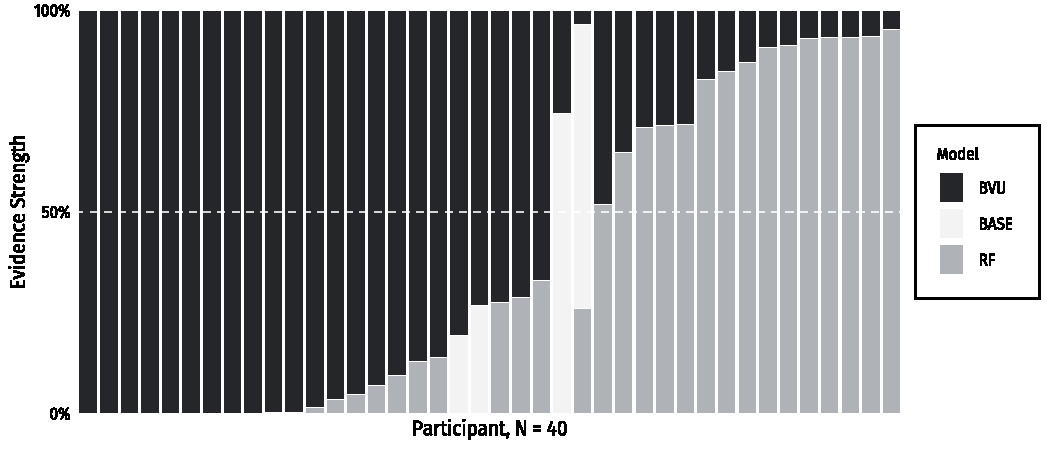
\includegraphics[width=.9\linewidth]{../figures/fig2-1} 

}

\caption{Study 1: Evidence for the models for individual participants. \textit{RF}$=$ relative frequency model, \textit{BVU}$=$ Bayesian value updating model, \textit{BASE}$=$ Baseline model.}\label{fig:fig2}
\end{figure}

\added[id=jj]{
The estimated parameter of the best-fitting models, which Table \ref{tab:study1_parameter} summarizes, reveal that the power utility exponent ($\alpha$) did not differ for the participants that were described by a Bayesian value updating strategy ($M_{\alpha}= 1.49$) and those using a relative frequency strategy ($M_{\alpha}=1.61$), $\Delta$ $M = -0.08$ 95\% HDI $[-0.97$, $0.76]$, $\mathrm{BF}_{\textrm{01}} = 2.76$. Participants using the Bayesian strategy had, on average, a prior belief that gains occur with 46\% (gain prior $\theta_G = 0.92$; zero-outcome prior $\theta_0 = 1.08$). Also, their estimated learning rate $\delta$ was anti-conservative ($M_{\delta}=1.36$; values $>$ 1 are liberal, 1 is optimal Bayesian, $<$ 1 is conservative learning). The liberal learning rate is unusual given that previous work has found conservative learning \citep{Edwards1967,Tauber2017}. The liberal learning in our data can be explained by that participants repeatedly sampled from the same set of gambles.
}

\begin{table}[tbp]

\begin{center}
\begin{threeparttable}

\caption{\label{tab:study1_parameter}Study 1: Parameter Estimates of Winning Models, \textit{M (SD)}}

\begin{tabular}{lccccc}
\toprule
Winning Model & $\alpha$ & $\delta$ & $\theta_G$ & $\mu$ & $\sigma$\\
\midrule
BVU (\textit{n}$=$30) & 1.49 (1.47) & 1.36 (2.12) & 0.92 (0.66) & -- & 0.13 (0.07)\\
RF (\textit{n}$=$9) & 1.61 (0.58) & -- & -- & -- & 0.12 (0.02)\\
BASE (\textit{n}$=$1) & -- & -- & -- & 0.47 (NA) & 0.30 (NA)\\
\bottomrule
\addlinespace
\end{tabular}

\begin{tablenotes}[para]
\normalsize{\textit{Note.} \textit{BVU}$=$ Bayesian value updating model, \textit{RF}$=$ relative frequency model, \textit{BASE}$=$baseline model. Parameters denote: $\alpha=$ power utility exponent, $\theta_G$ gain prior, $\mu=$ mean evaluation, $\sigma$ standard deviation.}
\end{tablenotes}

\end{threeparttable}
\end{center}

\end{table}

\textit{Qualitative Model Fit.} The qualitative fit between the models
and the data is shown in Figure \ref{fig:fig5}, which plots the
predictions of the best-fitting models against the observed evaluations
by participant. The models generally describe the data well
\added[id=jj]{($M r\textsubscript{pred,obs} = 0.71$), except in four cases, where even the winning model fails to resemble the data qualitatively (participants s05, s19, s24, s38, with $r\textsubscript{pred,obs} < 0.40$).}
For these cases, for whom the winning model is the Bayesian updating
model, the model must be rejected because of qualitative
mis-fit.\footnote{As robustness check we repeated the model comparison with subjective probability weighting, using Prelec’s single parameter weighting function. This weighting function incorporates non-linearities in the perception of probabilities. However, the quantitative results of the probability weighting model and the utility model, we favored a utility model without probability weighting.}

\begin{figure}[htb]

{\centering 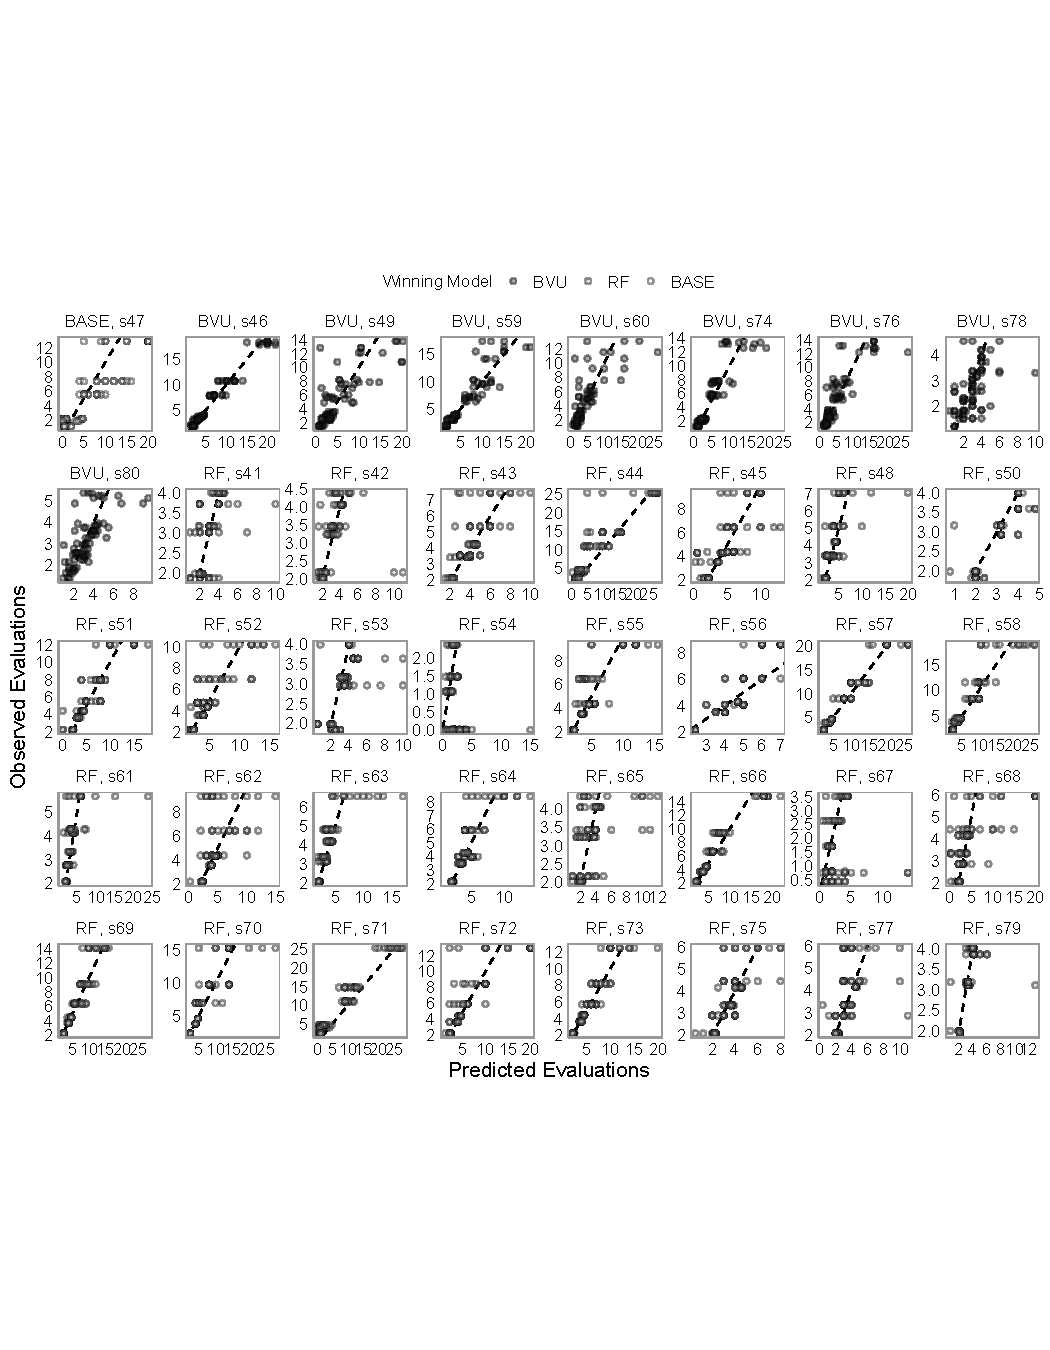
\includegraphics[width=\textwidth]{../figures/fig5-1} 

}

\caption{Study 1: Predicted evaluations from the best-fitting models plotted against the observed evaluations (by participant). \textit{BVU}$=$ Bayesian value updating model, \textit{RF}$=$ relative frequency model, \textit{BASE}$=$baseline model.}\label{fig:fig5}
\end{figure}

\added[id=jj]{
The cognitive modeling results thus show that most participants were described by a Bayesian strategy, and a minority by a relative-frequency strategy. This strategy heterogeneity helps understanding the behavioral null finding---that sample size seemed to have no effect on valuations---that were observed at the aggregate level (Table \ref{tab:means_study1}). The aggregate analysis fails to take the individual differences in learning strategies into account, while participants are best described by a mixture of strategies. Moreover, the aggregate analysis also fails to account for differences in the prior beliefs about gain probabilities.
}


\end{document}
